%!TEX root = ../thesis.tex
\chapter{Methods}
\label{chap:methods}

In Section \ref{sec:SAFT} the \ac{saft} is explained. Each voxel was assigned a value $V_k$ which was independent of the angle between the voxel and the emitter and receiver. During this process practically every directional information of the data is lost. 
To prevent this loss of information each \ac{ascan} has to be assigned a certain direction during the reconstruction.
For that the measurement volume and consequently each voxel has to be segmented. The multitude of directions is represented by a set of direction vectors. In principle the volume can be segmented into an arbitrary set of directions with a very high density of direction vectors. Since the amount of data that has to be processed increases with each additional direction vector the volume has to be divided in a sensible manner.


\section{Segmentation of the measurement volume}
\label{chap:segmentation}


The first step of the preservation of directional information during the reconstruction is the generation of a suitable set of direction vectors which divide the measurement volume as evenly as possible. Theoretically, the direction vectors do not have to be distributed equally. If a certain direction requires a higher resolution of the segmentation it would be no problem to either add more vectors to that particular direction or shift some existing vectors from a less relevant direction to that required direction. In the following it was aspired to distribute the vectors as evenly as possible since no information about the relevance of one certain direction over another are available during this thesis.
In Section \ref{chap:platonicsolids} platonic solids are used to generate a set of either 12 or 20 vectors which are equally distributed. The limitation of the amount of vectors which arises with the usage of platonic solids is tackled by the method in Section \ref{chap:arbitrarySegment}.



\subsection{Platonic solids}
\label{chap:platonicsolids}

Since the goal of the segmentation is to divide the measurement volume of each voxel as evenly as possible the intermediate angle between two neighbouring segmentation vectors should be equal.Platonic solids are one possibility to get a set of vectors which fulfil this requirement.
\begin{figure}[H]
     \centering
     \begin{subfigure}[b]{0.19\textwidth}
         \centering
        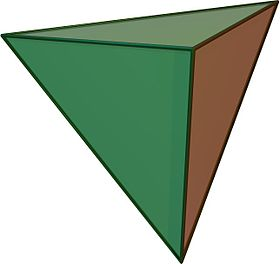
\includegraphics[width=0.8\linewidth]{Tetrahedron.jpg}
         \caption{Tetrahedron}
         \label{fig:Tetrahedron}
     \end{subfigure}
     \hfill
     \begin{subfigure}[b]{0.19\textwidth}
         \centering
         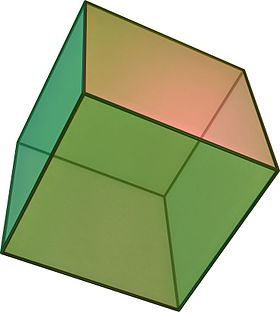
\includegraphics[width=0.87\textwidth]{cube.jpg}
         \caption{Cube}
         \label{fig:cube}
     \end{subfigure}
     \hfill
     \begin{subfigure}[b]{0.19\textwidth}
         \centering
         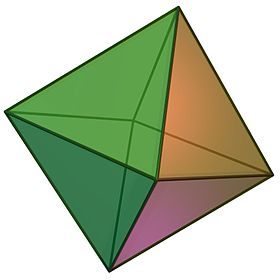
\includegraphics[width=0.8\textwidth]{280px-Octahedron.jpg}
         \caption{Octahedron}
         \label{fig:Octahedron}
     \end{subfigure}
     \hfill
     \begin{subfigure}[b]{0.19\textwidth}
         \centering
         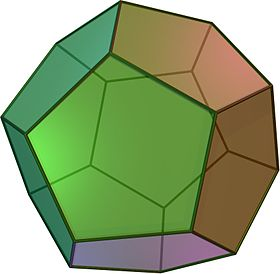
\includegraphics[width=0.93\textwidth]{280px-Dodecahedron.jpg}
         \caption{Dodecahedron}
         \label{fig:Dodecahedron}
     \end{subfigure}
     \hfill
     \begin{subfigure}[b]{0.19\textwidth}
         \centering
         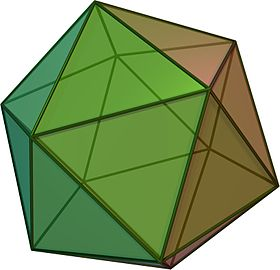
\includegraphics[width=0.8\textwidth]{280px-Icosahedron.jpg}
         \caption{Icosahedron}
         \label{fig:Icosahedro}
     \end{subfigure}
        \caption{The five platonic solids. They all have equally sized faces. Picture source: \cite{wiki_platonic}}
        \label{fig:platonic_solids}
\end{figure}

A key feature of platonic solids are the equally sized faces and therefore the evenly distributed face normals if placed in the centre of each face.
There are five different platonic solids (shown in Fig. \ref{fig:platonic_solids}): The tetrahedron with four faces, the cube with six faces, the octahedron with eight faces, the dodecahedron with 12 faces and the icosahedron with 20 faces.
From these five platonic solids the dodecahedron as well as the icosahedron are currently used to generate suitable segmentation vectors. Theoretically, the remaining geometries provide a suitable set of evenly distributed normals for the segmentation of the volume as well. Since they only have eight or less faces the comparably low resolution of the segmentation of the volume would make an analysis of the direction of propagation rather difficult.

\bigskip

Figure \ref{fig:Dodecahedron_MATLAB} shows the implementation of the dodecahedron in MATLAB. Each face normal as well as the corresponding index is plotted in the centre of each face. Figure \ref{fig:Icosahedron_MATLAB} shows the icosahedron.

\begin{figure}[H]
     \centering
     \begin{subfigure}[b]{0.47\textwidth}
         \centering
        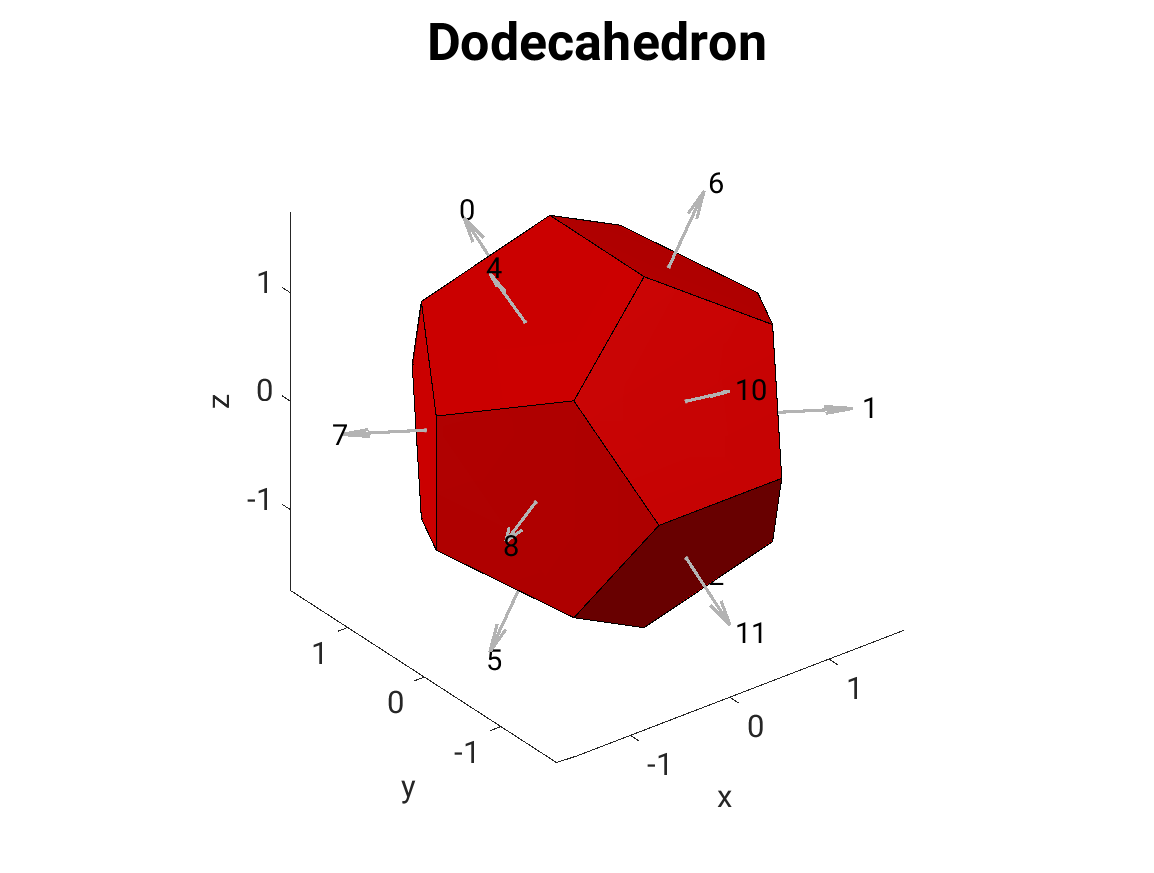
\includegraphics[width=1.2\linewidth]{Graphics/Dodecahedron.eps}
         \caption{Dodecahedron with 12 faces and 12 face normals.}
         \label{fig:Dodecahedron_MATLAB}
     \end{subfigure}
     \hfill
     \begin{subfigure}[b]{0.47\textwidth}
         \centering
         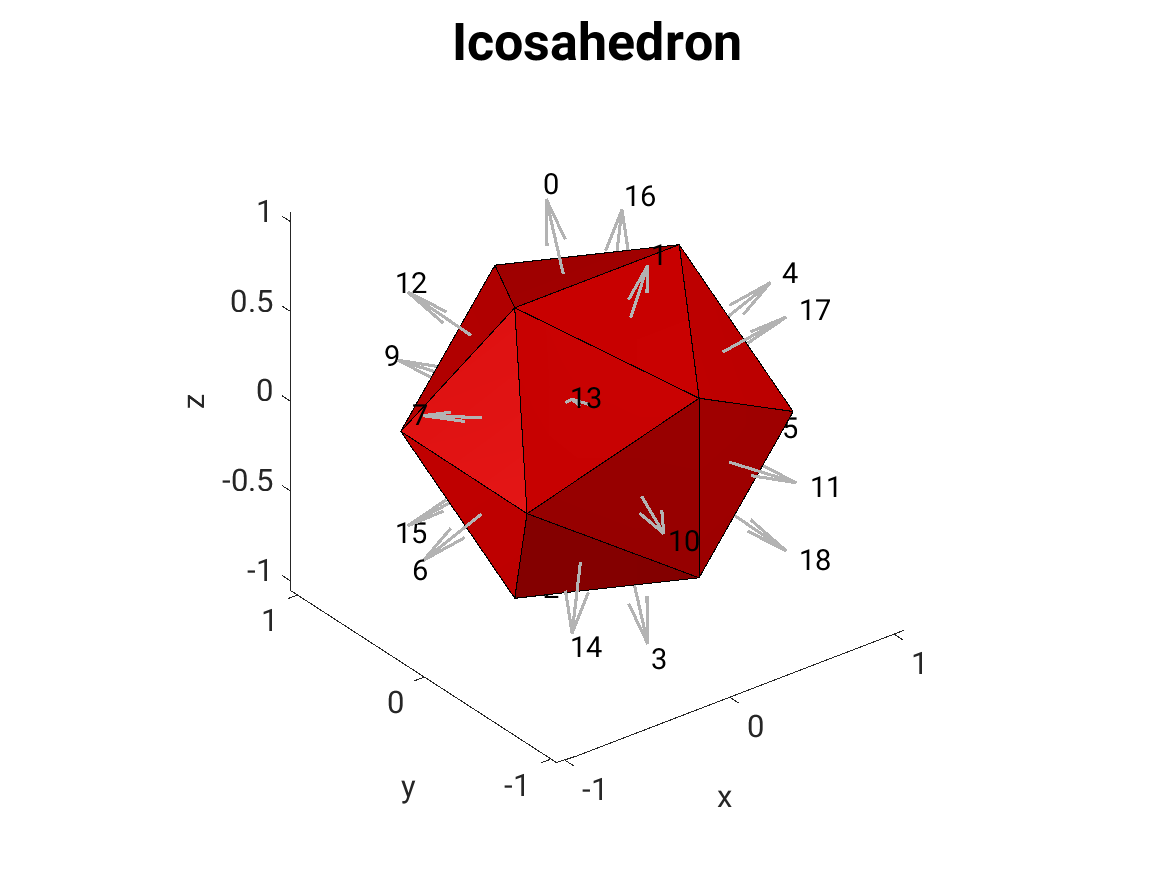
\includegraphics[width=1.2\textwidth]{Graphics/Icosahedron.eps}
         \caption{Icosahedron with 20 faces and 20 face normals.}
         \label{fig:Icosahedron_MATLAB}
     \end{subfigure}
        \caption{Both platonic solids realised in MATLAB. In the centre of each face the normal vector is plotted with its corresponding index. }
        \label{fig:platonic_solids_matlab}
\end{figure}


\subsection{Arbitrary Segmentation}
\label{chap:arbitrarySegment}


\subsection{Gradnetz}




\section{Identification of faces}
For the analysis of the direction-dependent reflection characteristics each \ac{ascan} has to be assigned to a certain direction of the voxel.
Depending on which geometry was chosen for the segmentation of the volume there is a set of normals which are orthogonal to each face of the geometry. To assign a face to each \ac{ascan} it makes sense to calculate the angle $\angle (\overrightarrow{a},\overrightarrow{b})$ between the direction vector and each normal.


\begin{equation}
\centering
\angle (\overrightarrow{a},\overrightarrow{b}) = \varphi
\label{eqation_angle}
\end{equation}


\begin{equation}
\centering
cos(\varphi )  =   \frac{(\overrightarrow{a} \cdot \overrightarrow{b})}{\left \| \overrightarrow{a} \right \|_2  \cdot \left \| \overrightarrow{b} \right \|_2}
\label{eqation_cos_phi}
\end{equation}

\begin{equation}
\angle (\overrightarrow{a},\overrightarrow{b}) = 
cos^{-1} \left (  
\frac{(\overrightarrow{a} \cdot \overrightarrow{b})}{\left \| \overrightarrow{a} \right \|_2  \cdot \left \| \overrightarrow{b} \right \|_2} 
\right )
\label{eqation_angle_final}
\end{equation}

To identify the face which belongs to the corresponding \ac{ascan} the smallest angle of the set has to be found.

\qquad





For every emitter-receiver combination, for each voxel and each rotation position of the aperture one calculation of the angle between two vectors has to be performed. Depending on which geometry is used for every normal of the faces of the geometry this calculation hast to be repeated. The number of calculations results in:

\boxed{ \# Calculations = \#Voxel \cdot \#Emitter \cdot \#Receiver \cdot \#AperturRotation \cdot \#Faces}

For the case of using a 12 face dodecahedron, 628 emitters, 1413 receivers, only a single slice of 1024x64 voxels and ten aperture positions already $[628 \cdot 1413 \cdot 1024 \cdot 64 \cdot 10 \cdot 12] = 6.98x10^{12}$ calculations have to be  performed to find the smallest angle index. By decreasing the complexity of these calculations the performance of the reconstruction algorithm can be greatly improved. To reduce the computational cost it is not necessary to calculate the absolute angle between each vector combination. It simply can be proven that for certain circumstances one certain combination of direction vector and face-normal has the smallest angle of the available set. The following segment is adapted from \cite{PatrickHucker2014EvaluationRuckstreumodells} and some inaccuracies were corrected.

\qquad

In the following $\overrightarrow{v}$ is the direction vector from the \ac{ascan} which should be matched best to one of the norm vectors $\overrightarrow{n_i}$ from the $N$ faces of the used geometry.


\begin{equation}
\angle (\overrightarrow{v},\overrightarrow{n_i}) =  cos^{-1}\left (    \frac{(\overrightarrow{v} \cdot \overrightarrow{n_i})}{\left \| \overrightarrow{v} \right \|_2  \cdot {\left \| \overrightarrow{n_i} \right \|_2}}  \right ) 
\label{equation_with_v_n}
\end{equation}



For the first simplification we can neglect the $arccos$ in equation \ref{equation_with_v_n}. Since the arccosine is monotonically decreasing in the interval $[-1,1]$ (Figure \ref{accos_figure}) only the argument of the $arccos$ has to be regarded to find the smallest angle $\angle (\overrightarrow{v},\overrightarrow{n_i})$. To reach a small value for the arccosine function its argument has to become as big as possible.
\begin{equation}
min \left (  \angle (\overrightarrow{v},\overrightarrow{n_i}) \right ) =  max \left (    \frac{(\overrightarrow{v} \cdot \overrightarrow{n_i})}{\left \| \overrightarrow{v} \right \|_2  \cdot {\left \| \overrightarrow{n_i} \right \|_2}}  \right ) 
\label{equation_acos_neglect}
\end{equation}

\begin{figure}[H]
    \centering
    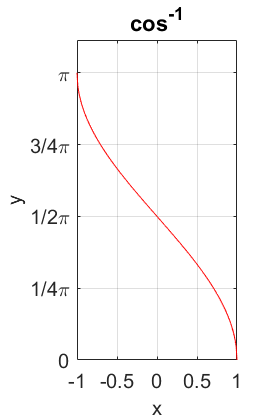
\includegraphics[width=0.3\textwidth]{accos.png}
    \caption{ Monotonically decreasing arccosine function.}
    \label{accos_figure}
\end{figure}

Since the euclidean norm of a normal vector $\left \| \overrightarrow{n_i} \right \|_2 = 1 , \forall i \in [1,...,N]$, the equation \ref{equation_acos_neglect} can be simplified further:


\begin{equation}
min \left (  \angle (\overrightarrow{v},\overrightarrow{n_i}) \right ) =  max \left (    \frac{(\overrightarrow{v} \cdot \overrightarrow{n_i})}{\left \| \overrightarrow{v} \right \|_2  \cdot { \underset{=1}{\underbrace{\left \| \overrightarrow{n_i} \right \|_2}}} }  \right ) = 
max \left (    \frac{(\overrightarrow{v} \cdot \overrightarrow{n_i})}{\left \| \overrightarrow{v} \right \|_2  }  \right )
\label{equation_acos_norm_simply}
\end{equation}

During the search of the smallest angle between the direction vector $\overrightarrow{v}$ and the set of normal vectors $\overrightarrow{n_i}$ the direction vector $\overrightarrow{v}$ does not change. 
The norm of the direction vector $\left \| \overrightarrow{v} \right \|_2$ is the same in every iteration of the search, thus has no influence on the final result and therefore can be remove from the formula.

\begin{equation}
min \left (  \angle (\overrightarrow{v},\overrightarrow{n_i}) \right ) = 
max \left (    \frac{(\overrightarrow{v} \cdot \overrightarrow{n_i})}{\left \| \overrightarrow{v} \right \|_2  }  \right ) = max \left (    \overrightarrow{v} \cdot \overrightarrow{n_i}  \right ) 
\label{equation_other_norm_simply}
\end{equation}

The final problem arises from equation \ref{equation_other_norm_simply}. The goal is to find the index $i_0$ for which the product of the direction vector $\overrightarrow{v}$ and the normal $\overrightarrow{n_{i_0}}$ is maximised: 

\begin{equation}
i_0 = \underset{i \in 0..N}{\mathrm{argmax}} \left (    \overrightarrow{v} \cdot \overrightarrow{n_i}  \right )
\label{equation_arg_max}
\end{equation}



\subsection{Orthogonality}
For the analysis of the direction-dependent reflection characteristics each \ac{ascan} has to be assigned to a certain direction of the voxel.
In chapter \ref{chap:segmentation} the methods for the segmentation of the volume were explained. Either the geometrical approach with the platonic solids or the arbitrary segmentation was chosen for the segmentation of the volume. In either case there is a set of equally distributed vectors which divide the volume into multiple segments. To assign the \ac{ascan} to a certain direction the orthogonality provides a good metric since the orthogonality is independent of the azimuth rotation direction between two vectors $\overrightarrow{a}$ and $ \overrightarrow{b}$. 
To get a conclusive result concerning the angular relation of two vectors one requirement of this method is that every vector has to be normalised. The length of each vector affects the scalar product and with that the orthogonality of the vector pair.
If this requirement is met one can arrive at the following:

Two vectors $\overrightarrow{a}$ and $\overrightarrow{b}$ are considered orthogonal to each other if the following assumption is fulfilled:

\begin{equation}
\overrightarrow{a} \perp  \overrightarrow{b} \Leftrightarrow  \overrightarrow{a} \cdot  \overrightarrow{b} = 0
\label{equation_orthogonality}
\end{equation}


As an example the distribution of the orthogonality between the vectors $\overrightarrow{a}$ and $\overrightarrow{b}$  is shown in Figure \ref{orthogonaltiy_figure}. Vector $\overrightarrow{a} = \begin{bmatrix} 0 \\ 1 \end{bmatrix}$ is represented by the green arrow on the left side. It serves as a constant reference vector. On the right side there are three possible vectors $\overrightarrow{b}$ shown.

\begin{figure}[H]
    \centering
    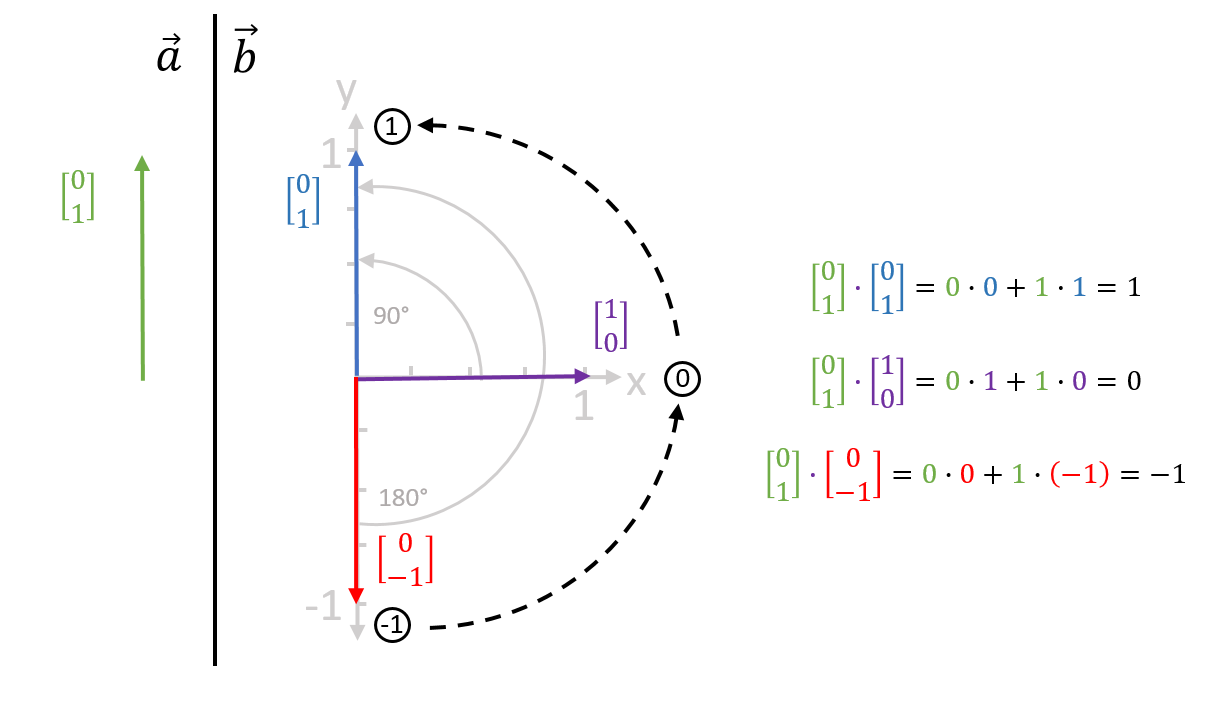
\includegraphics[width=0.8\textwidth]{Graphics/orthogonality.png}
    \caption{Example for the calculation of the orthogonality of one static reference vector$\overrightarrow{a}$ on the left side and three possible candidates for $\overrightarrow{b}$ on the right. The calculation show the transition of the orthogonality from its minimum at $-1$ to the maximum at $1$.}
    \label{orthogonaltiy_figure}
\end{figure}

The calculations on the right side of Figure \ref{orthogonaltiy_figure} show the orthogonality between each combination of $\overrightarrow{a}$ and $\overrightarrow{b}$. For example vector $\overrightarrow{a}$ and the purple vector $\overrightarrow{b}$ are perpendicular to each other. The calculations show that the orthogonality between both is zero and therefore fulfil the requirement of Equation \ref{equation_orthogonality}. The red vector $\overrightarrow{b}$ and the green comparison vector $\overrightarrow{a}$ comprise an angle of $180^{\circ}$ and therefore both vectors are pointing in the exact opposite direction. This results in an orthogonality of minus one.
If the vector $\overrightarrow{b}$ is pointing in the same direction as vector $\overrightarrow{a}$ they are parallel and the orthogonality between both is one. The dotted semicircle shows the transition of the orthogonality from its minimum to its maximum. In this interval the orthogonality monotonically increases non-linearly from $-1$ to $1$. An example of the non-linearity of the orthogonality is given in Figure \ref{orthogonaltiy_figure2}:

\begin{figure}[H]
    \centering
    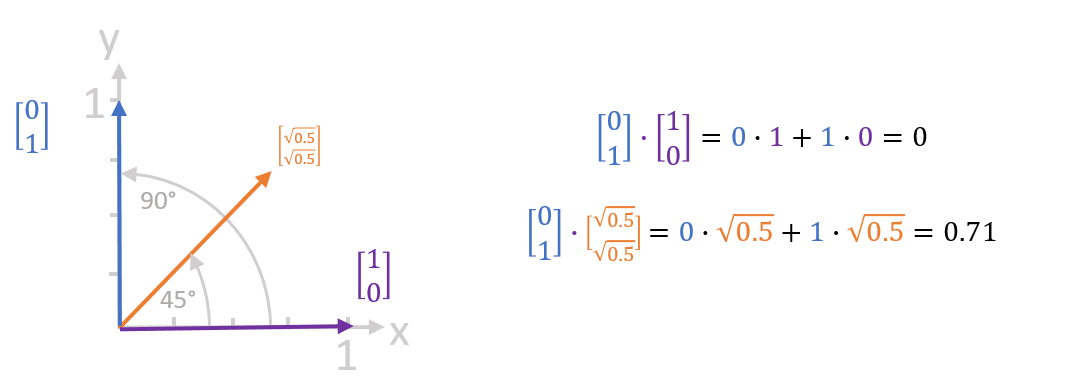
\includegraphics[width=0.8\textwidth]{Graphics/orthogonality2.png}
    \caption{Example of the non-linearity of the orthogonality in the interval $[-1,1]$. }
    \label{orthogonaltiy_figure2}
\end{figure}

The orthogonality between the blue vector $\begin{bmatrix} 0 \\ 1 \end{bmatrix}$ and the purple vector $\begin{bmatrix} 1 \\ 0 \end{bmatrix}$ is zero since both are perpendicular. The normalised bisector in between is shown by the orange vector.
The orthogonality between the blue vector and the bisector is approximately $0.71$ which shows the non-linear behaviour of the orthogonality which otherwise would have resulted in an orthogonality of $0.5$.





\section{Assignment of data to the segmentation vectors}
\label{sec:assigment}




\section{Performance evaluation}
To quantify how much overhead is generated by the additional calculation of the angle index.....




\begin{gather*}
Centered
\end{gather*} 